\section{Images}\label{sec:images}
\begin{figure}[H]
    \centering
    \begin{subfigure}{.5\textwidth}
        \centering
        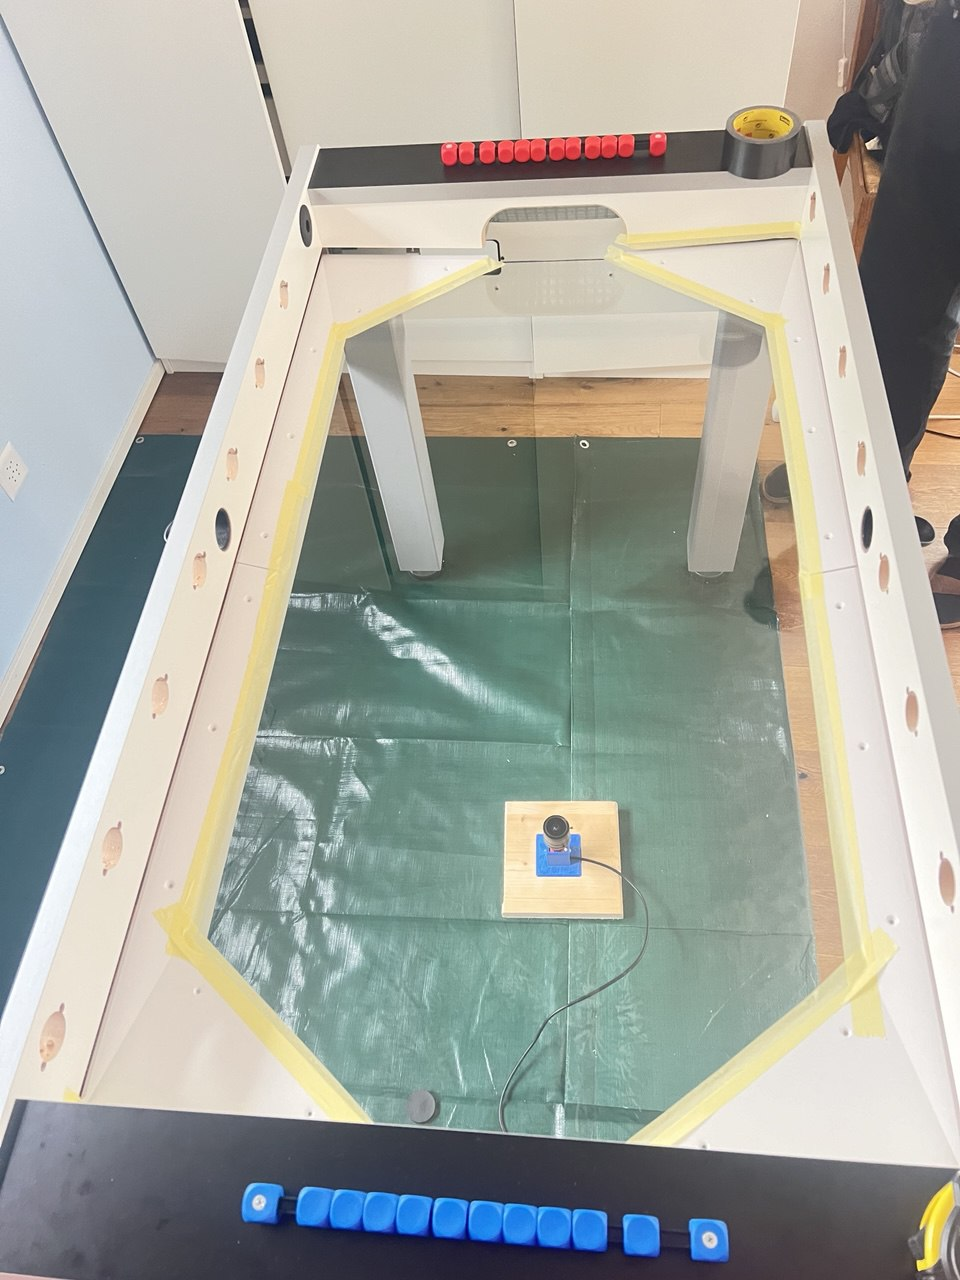
\includegraphics[width=0.9\linewidth]{../photos/glass_table}
        \caption{Foosball table with glass floor}
        \label{fig:glass_table}
    \end{subfigure}%
    \begin{subfigure}{.5\textwidth}
        \centering
        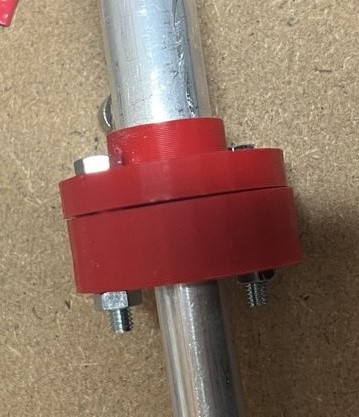
\includegraphics[width=0.9\linewidth]{../photos/connector_tube}
        \caption{Connection on the shoot side}
        \label{fig:connector_tube}
    \end{subfigure}
\end{figure}


\section{CNN}\label{sec:cnn}

\subsection{CNN architecture}\label{subsec:cnn-architecture}

\begin{figure}[H]
    \centering
    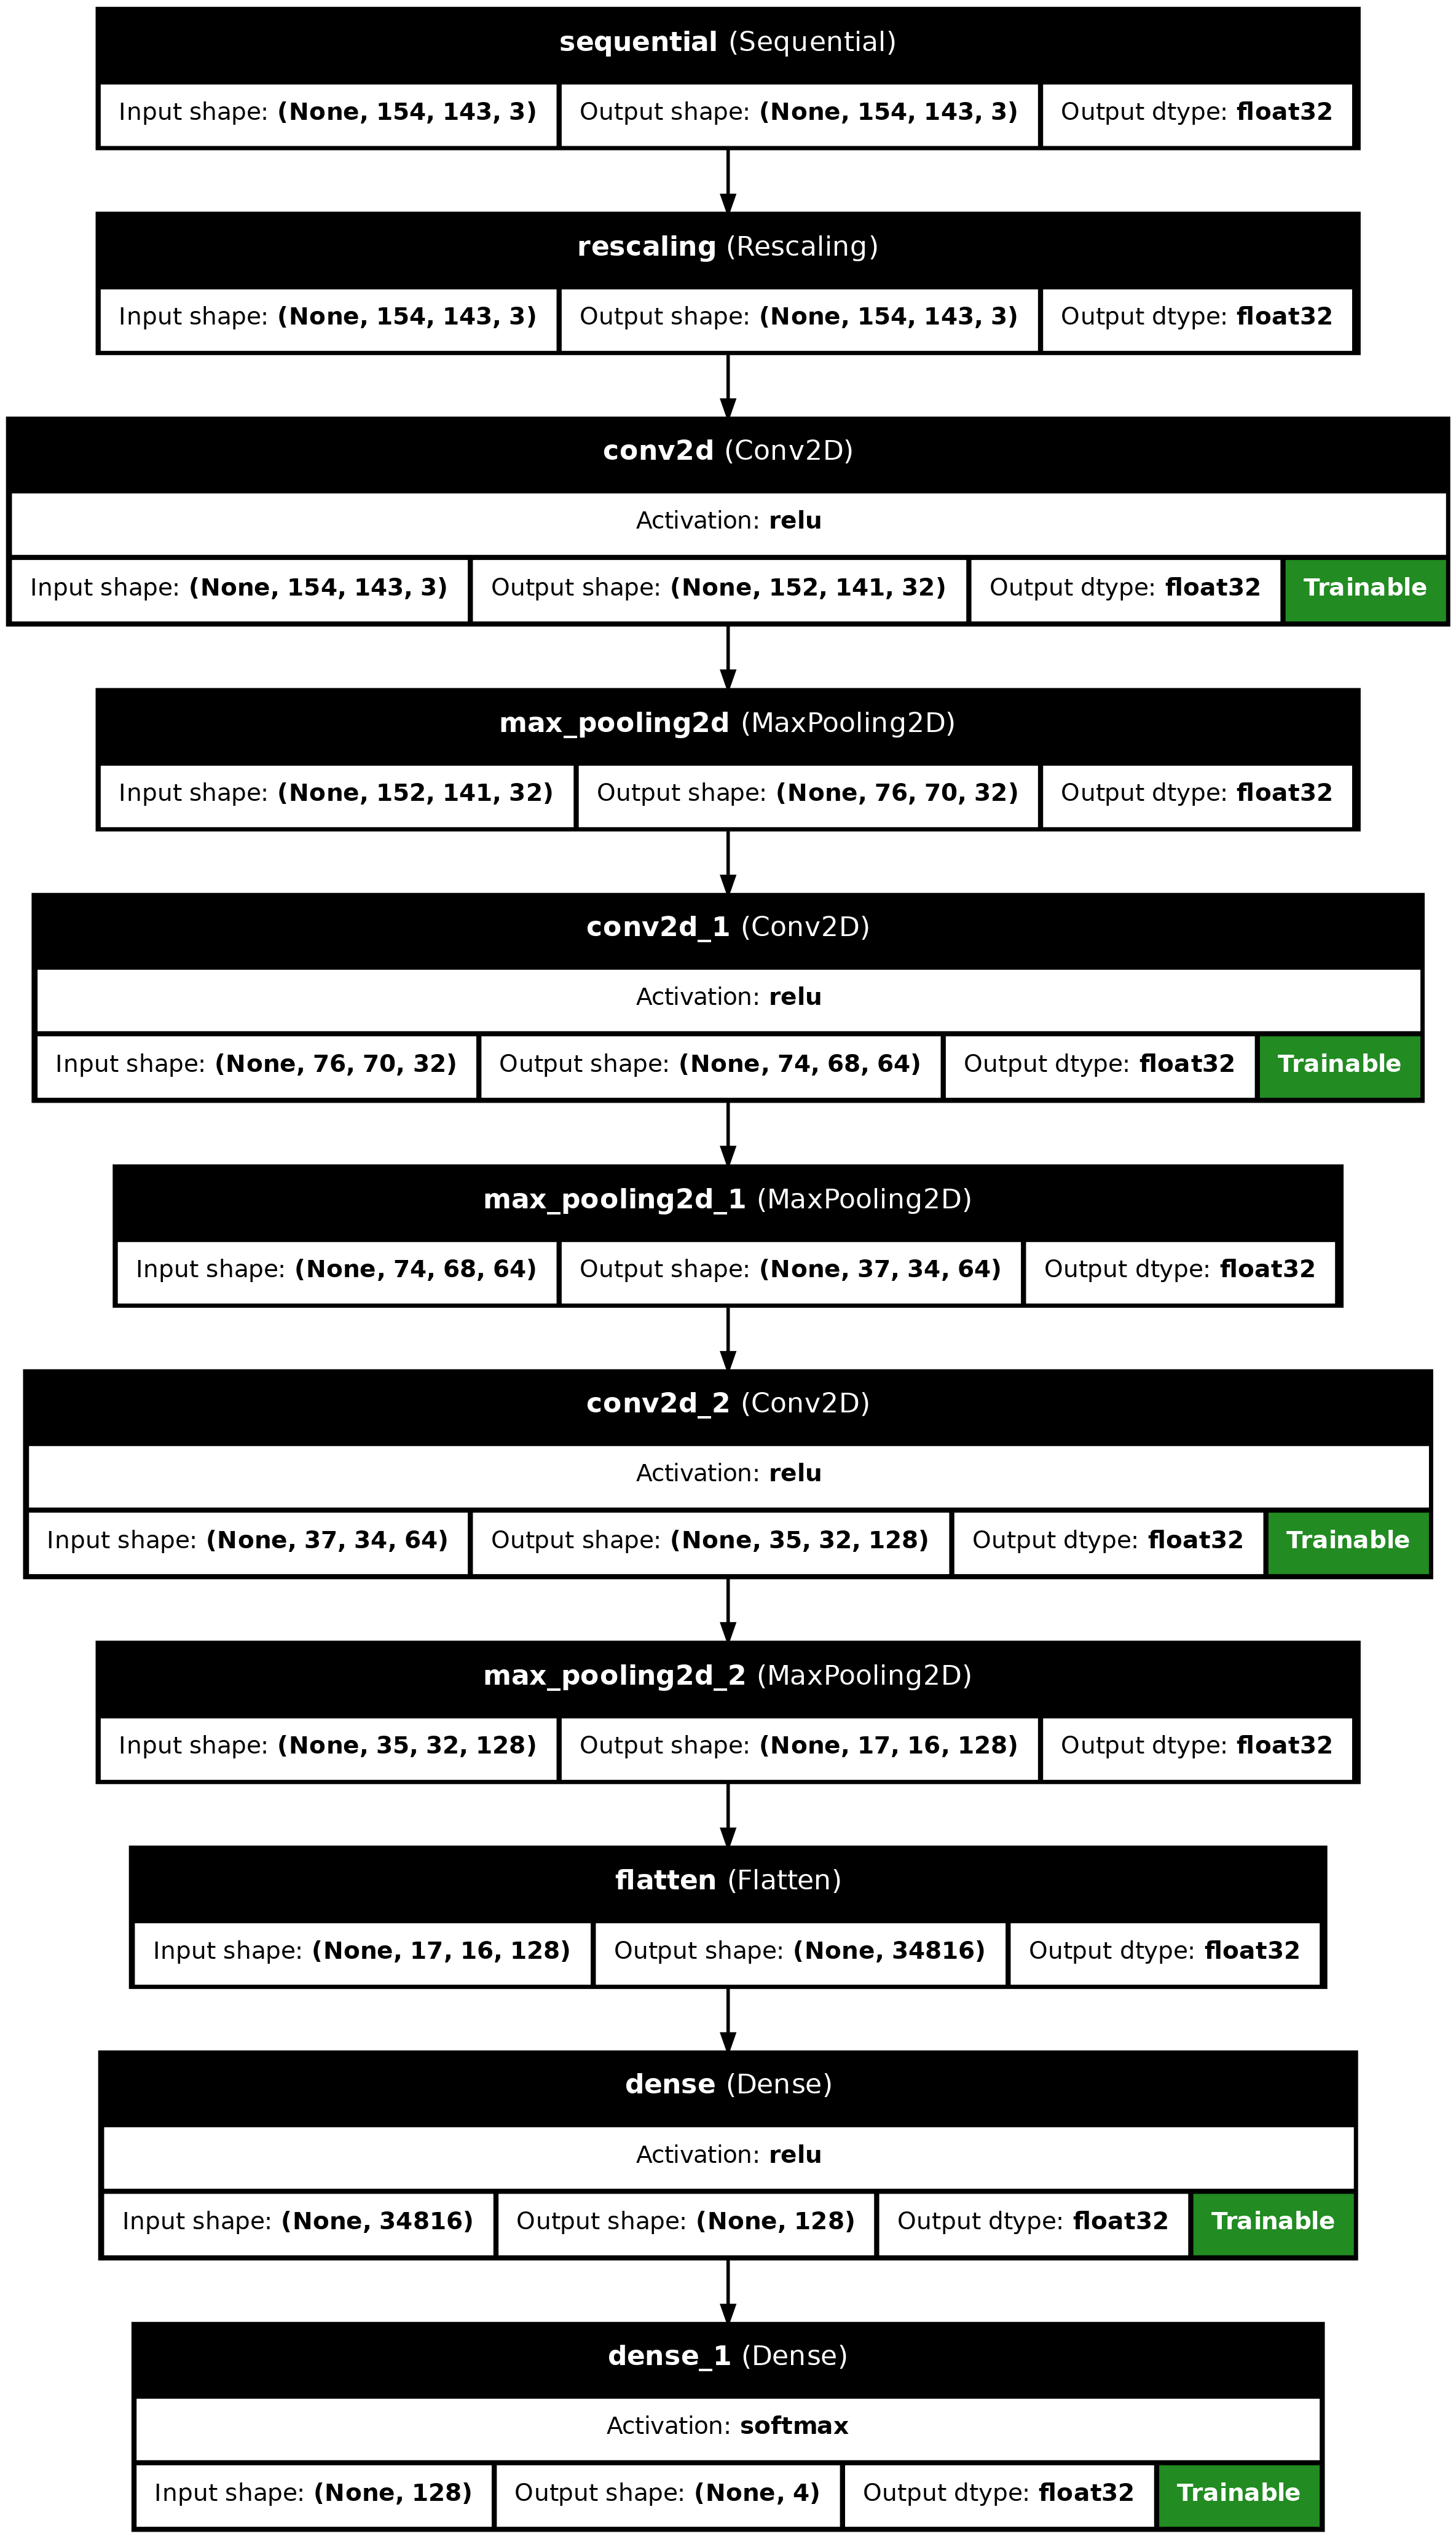
\includegraphics[height=.7\paperheight]{../photos/fiducial_classifier_model}
    \caption[originalRainbow]{Fiducial classifier model}
    \label{fig:fiducial_classifier_model}
\end{figure}
\begin{figure}[H]
    \centering
    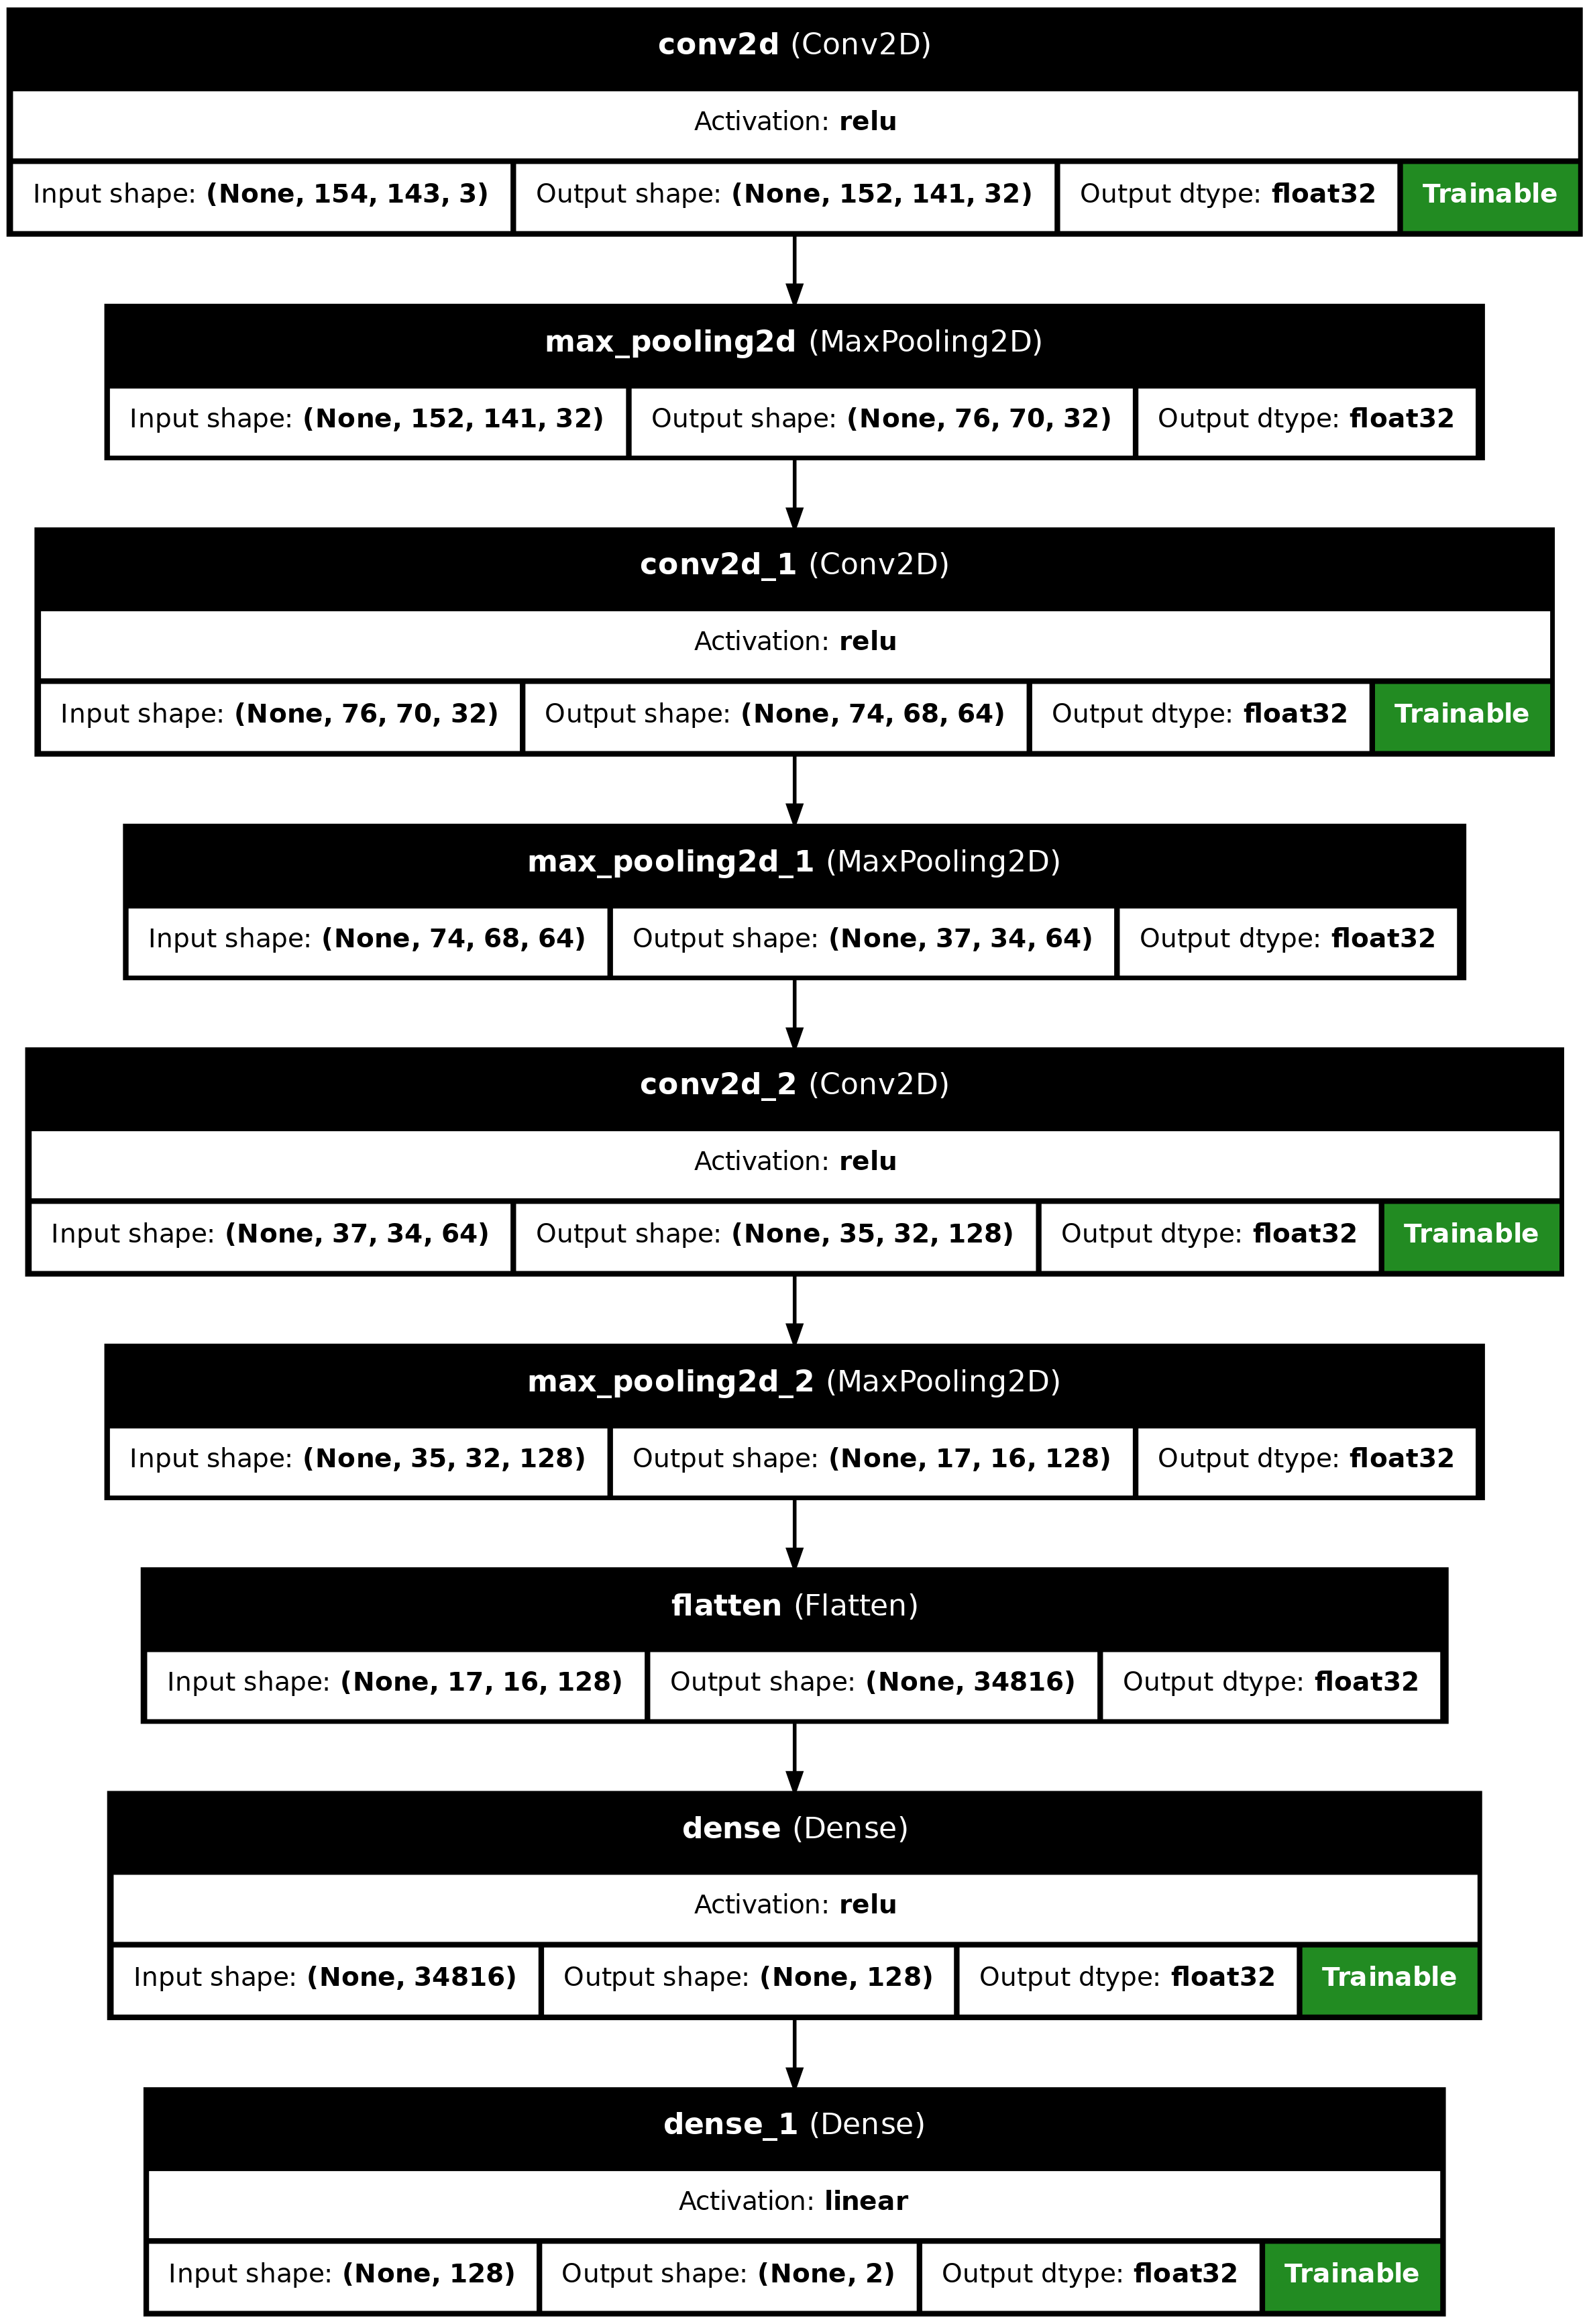
\includegraphics[height=.8\paperheight]{../photos/fiducial_coords_model}
    \caption[originalRainbow]{Fiducial coordinates model}
    \label{fig:fiducial_coords_model}
\end{figure}
\newpage

\subsection{Grad-CAM}\label{subsec:gradcam}
\begin{figure}[!ht]
    \centering
    \includegraphics[width=\textwidth]{../photos/gradcam_combined_image}
    \caption[originalRainbow]{Grad-CAM of all the layers in the fiducial coordinates model}
    \label{fig:gradcam}
\end{figure}


\section{Whole flowchart}\label{sec:whole-flowchart}

\begin{center}
    \begin{tikzpicture}[node distance=2cm]
        \node (cam) [io] {Camera};
        \node (undistortion) [process, below of=cam] {Undistortion};
        \node (ball_detection) [process, below of=undistortion] {Ball detection};
        \node (prediction) [process, below of=ball_detection] {Prediction};
        \node (where) [process, below of=prediction, right of=prediction, xshift=1.5cm] {Where?};
        \node (when) [process, below of=prediction, left of=prediction, xshift=-1.5cm] {When?};
        \node (arduino) [process, below of=when, right of=when, xshift=1.5cm] {Arduino};
        \node (cnc) [process, below of=arduino, right of=arduino, xshift=1.5cm] {CNC shield};
        \node (cnc-text)  [above of=cnc, yshift=-1cm] {Target player position};
        \node (drv) [process, below of=cnc] {DRV8825};
        \node (stepper) [io, below of=drv] {Stepper Motor};
        \node (stepper-text) [below of=stepper, yshift=1cm] {Move side};
        \node (l298n) [process, below of=arduino, left of=arduino, xshift=-1.5cm] {L298N};
        \node (shoot-text)  [above of=l298n, yshift=-1cm] {Shoot the ball};
        \node (dc) [io, below of=l298n] {DC Motor};
        \node (dc-text) [below of=dc, yshift=1cm] {Shoot side};

        % arrows
        \draw [arrow] (cam) -- (undistortion);
        \draw [arrow] (undistortion) -- (ball_detection);
        \draw [arrow] (ball_detection) -- (prediction);
        \draw [arrow] (prediction) |- (where);
        \draw [arrow] (prediction) |- (when);
        \draw [arrow] (where) |- (arduino);
        \draw [arrow] (when) |- (arduino);

        \draw [arrow] (arduino) |- (cnc);
        \draw [arrow] (cnc) -- (drv);
        \draw [arrow] (drv) -- (stepper);
        \draw [arrow] (arduino) |- (l298n);
        \draw [arrow] (l298n) -- (dc);


        \coordinate (corner1) at ([xshift=-0.3cm]when.west |- undistortion.north);


%        make box around undistortion and ball_detection as they are on the computer
        \draw[red,thick] ($(where.south east)+(0.3,-0.3)$) rectangle ([xshift=-0.3cm, yshift=0.3cm]when.west |- undistortion.north) node[above, xshift=2cm] {Software (Chapter~\ref{ch:software})};
%       make box from l298n to stepper
        \draw[red,thick] ($(l298n.north west)+(-1,2.3)$)  rectangle ($(stepper.south east)+(2.3,-0.9)$) node[below,midway, yshift=-4cm] {Electronics (cf. Chapter~\ref{ch:electronics})};
    \end{tikzpicture}
\end{center}


